\subsection{Factorisation et résolution triangulaire}
Le parallélisme de la factorisation ILU et de la résolution triangulaire est le même.
%
La résolution triangulaire peut donc réutiliser le graphe grossier calculé pour la factorisation.
%
La fonction exécutée à l'intérieur des tâches sera différente, dans un cas il s'agira de factoriser une ou plusieurs lignes de la matrice, et dans l'autre cas il s'agira de résoudre une ou plusieurs équations linéaires à une inconnue.



Les pages mémoires composant la matrice sont distribuées en respectant l'affinité mémoire des tâches associées.
%
Taggre a défini cette affinité en distribuant les tâches sur les bancs NUMA en équilibrant le nombre de pages par banc NUMA pour chaque hauteur du graphe.
%
Nous avons ainsi une distribution à peu près équitable des pages mémoires au fil du déroulement du graphe.
%
Le même mécanisme qui sert à utiliser un seul graphe de tâches pour la factorisation et la résolution triangulaire est utilisé ici pour choisir les pages mémoires à déplacer.
%
Pour cela, le programmeur doit créer une fonction qui enregistre auprès de Taggre les données utilisées, cette fonction sera celle exécutée par toutes les tâches du graphe.
%
Puis Taggre s'occupera d'optimaliser le placement des pages mémoires en effectuant les appels systèmes correspondants.
%
Malheureusement, nous ne pouvons pas distribuer toutes les pages de manière optimale, car il arrive que certaines pages soient utilisées par plusieurs tâches ayant des affinités mémoires différentes.
%
Dans un tel cas, nous choisissons de placer la page mémoire sur le banc NUMA ayant le plus de tâches.

% -------------------------------
\subsubsection{Mémoire distribuée}
En mémoire distribuée, nous utilisons une méthode de Jacobi par blocs pour obtenir du parallélisme.
%
Chaque processus factorise un bloc de la matrice en parallèle.
%
Nous n'effectuons donc pas le même calcul que lors d'une factorisation en mémoire partagée.
%
Il y a un peu plus de calcul à faire en mémoire partagée, ces calculs correspondent aux éléments en dehors des blocs qui sont ignorés avec la méthode de Jacobi par blocs.
%
Par contre, cette méthode nous permettra d'évaluer une borne maximale de performances que nous pourrons obtenir en mémoire partagée.
%
En effet, les types d'opérations sont les mêmes, seul l'ordre de traitement des lignes de la matrice change avec l'ajout de dépendances entre chaque ligne.


Sur la machine Rostand, la factorisation ILU(0) atteint une accélération de 9,9 (Fig.~\ref{fig:res_facto_mpi_rostand}) et la résolution triangulaire une accélération de 3,7 sur 12 coeurs de calcul (Fig.~\ref{fig:res_trsv_mpi_rostand}).
%
La factorisation est moins limitée par la bande passante mémoire que la résolution triangulaire.
%
Sur la machine Manumanu, cette accélération monte à 93 pour la factorisation (Fig.~\ref{fig:res_facto_mpi_manu}) et à 73 pour la résolution triangulaire (Fig.~\ref{fig:res_trsv_mpi_manu}) pour 160 coeurs de calcul.
%
Si nous n'utilisons que deux processeurs de 8 coeurs de calcul chacun sur Manumanu, nous obtenons des accélérations de 15,18 pour la factorisation et 7,2 pour la résolution triangulaire.
%
Nous pouvons donc voir que la résolution triangulaire passe mieux à l'échelle que la factorisation.


\subsubsection{First touch}
Nous allons maintenant tester la politique d'allocation first touch sur la factorisation et sur la résolution triangulaire.
%
Les matrices et les vecteurs seront donc alloués sur un seul banc NUMA, celui du thread qui a exécuté le code d'initialisation.
%
Tous les accès mémoire passeront ensuite par ce banc NUMA, nous n'utiliserons donc qu'une partie de la bande passante mémoire de la machine.
%
Nous avons aussi utilisé Taggre pour grossir le grain de calcul.


Sur la machine Rostand, nous obtenons au mieux une accélération de 8,7 (Fig.~\ref{fig:res_facto_ft_rostand}) sur 12 coeurs pour la factorisation et une accélération de 2,8 pour la résolution triangulaire (Fig.~\ref{fig:res_trsv_ft_rostand}).
%
Nous obtenons donc des performances en dessous des performances obtenues en mémoire distribuée.
%
Il faut aussi prendre en compte que l'utilisation de plusieurs threads implique une gestion des dépendances entre les tâches de calcul.


Sur la machine Manumanu, nous obtenons le même type d'accélération que pour le produit matrice vecteur creux.
%
Tant que nous utilisons moins de 2 bancs NUMA, nous obtenons une accélération de 10 pour la factorisation (Fig.~\ref{fig:res_facto_ft_manu}) et une accélération de 6,2 pour la résolution triangulaire (Fig.~\ref{fig:res_trsv_ft_manu}).
%
Au-delà de 16 threads, les performances chutent, les temps de latence des accès mémoires deviennent trop grands.


\subsubsection{Interleave}
Pour essayer de diminuer les effets NUMA, nous activons la politique d'allocation mémoire interleave.
%
Les pages mémoires sont donc distribuées uniformément entre chaque banc NUMA.
%
Nous pouvons donc utiliser plus de bande passante qu'avec l'allocation first touch précédente.


Sur Rostand, la factorisation donne des résultats légèrement moins bons qu'avec une politique d'allocation first touch (Fig.~\ref{fig:res_facto_inter_rostand})
%
Par contre, nous obtenons une amélioration entre 3~\% et 30~\% de la résolution triangulaire pour un nombre faible de variables primaires (Fig.~\ref{fig:res_trsv_inter_rostand}).
%
Même si nous avons la possibilité d'utiliser plus de bande passante mémoire, ce n'est pas pour cela qu'elle sera mieux utilisée.
%
En moyenne, la moitié des accès mémoire auront toujours une latence plus élevée.



Sur Manumanu, la factorisation se comporte de la même façon que sur Rostand (Fig.~\ref{fig:res_facto_inter_manu}).
%
De même, l'accélération maximale de la résolution triangulaire est meilleure avec une politique d'allocation interleave (Fig.~\ref{fig:res_trsv_inter_manu}).
%
Comme pour la politique first touch, après 16 threads, les performances chutent.


\subsubsection{NATaS}
\`A la différence des autres ordonnanceurs, NATaS va tenir compte de l'affinité NUMA des tâches.
%
Cette affinité a été définie par Taggre de telle sorte à équilibrer la charge sur les différents bancs NUMA.
%
Donc, nous limitons le nombre d'accès aux bancs NUMA distants.
%
La granularité de placement mémoire étant d'une page, il n'est pas possible d'allouer toutes les données correctement.
%
Certaines données seront donc à cheval sur deux bancs NUMA différents.
%
De plus, dans le cas de la résolution triangulaire, les vecteurs seront eux aussi à cheval sur plusieurs bancs NUMA.



NATaS offre de meilleures performances sur Rostand par rapport à la politique d'allocation interleave.
%
La factorisation est 40\% plus rapide avec 8 variables primaires (Fig.~\ref{fig:res_facto_nas_rostand}) et la résolution triangulaire est 23\% plus rapide (Fig.~\ref{fig:res_trsv_nas_rostand}).
%
Avec 1 variable primaire, nous n'obtenons pas de gain sur la résolution triangulaire.


Sur Manamanu, les résultats sont meilleurs qu'avec les précédentes allocations (Fig.~\ref{fig:res_facto_nas_manu} et \ref{fig:res_trsv_nas_manu}).
%
Par contre, au-delà de deux processeurs, les performances s'effondrent aussi.
%
Cette fois l'ordonnanceur en est la cause, les données sont bien réparties et chaque thread accède à des données locales.
%
Seul l'ordonnanceur accède à des données distantes pour des besoins de synchronisation.
%
Ces accès ne sont pas gênants dans un cas où la variation de latence est faible tels que deux processeurs dans un même groupe.
%
Mais cette variation devient gênante dès que l'on accède à un groupe NUMA distant.

% -------------------------------

%%%%%%%%%%%%%%%%
% Facto
%%%%%%%%%%%%%%%%
%   (-_-)   %
\begin{figure}[p]
     \begin{center}
        \subfigure[First touch.]{
          \label{fig:res_facto_ft_rostand}
          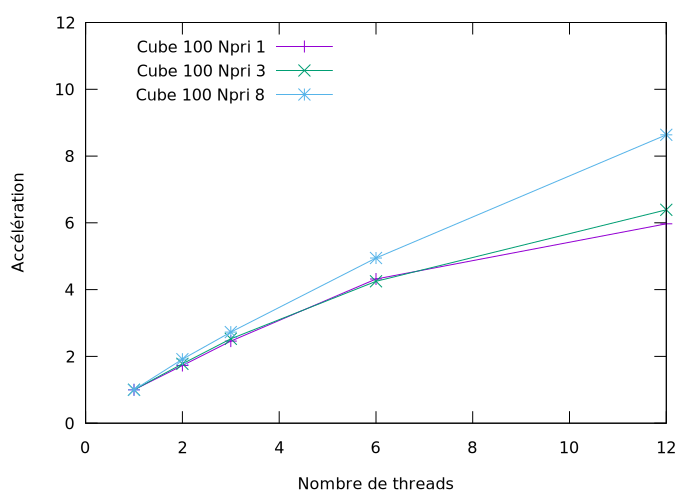
\includegraphics[width=0.48\textwidth]{res_facto_ft}
        }
        \subfigure[Interleave.]{
          \label{fig:res_facto_inter_rostand}
          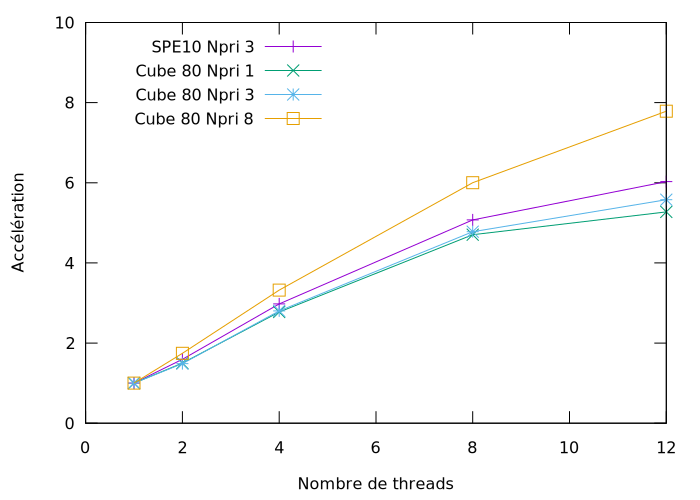
\includegraphics[width=0.48\textwidth]{res_facto_interleave}
        }
        \subfigure[NATaS.]{
          \label{fig:res_facto_nas_rostand}
          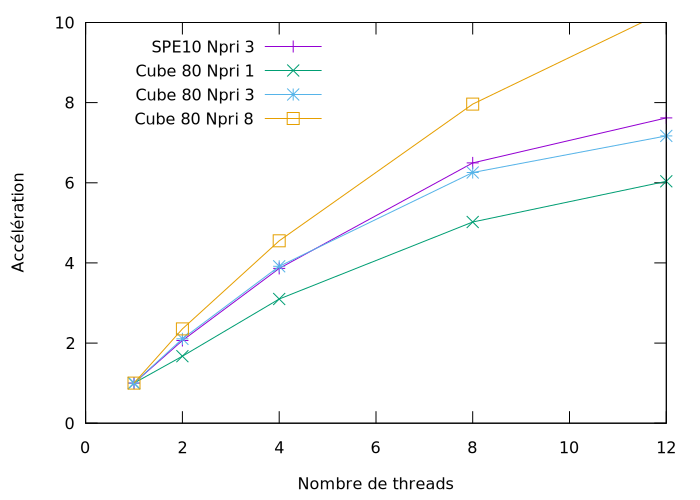
\includegraphics[width=0.48\textwidth]{res_facto_nas}
        }
        \subfigure[MPI.]{
          \label{fig:res_facto_mpi_rostand}
          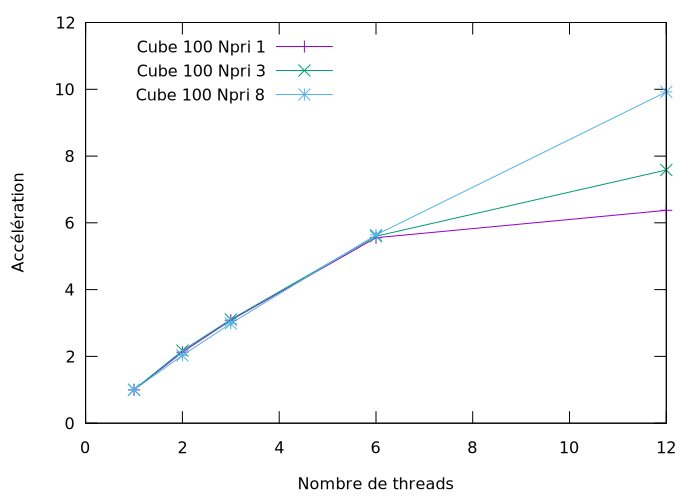
\includegraphics[width=0.48\textwidth]{res_facto_mpi_numa}
        }
    \end{center}
    \caption{Performances de la factorisation ILU(0) sur Rostand.}
\end{figure}

%   (-_-)   %
\begin{figure}[p]
     \begin{center}
        \subfigure[First touch.]{
          \label{fig:res_facto_ft_manu}
          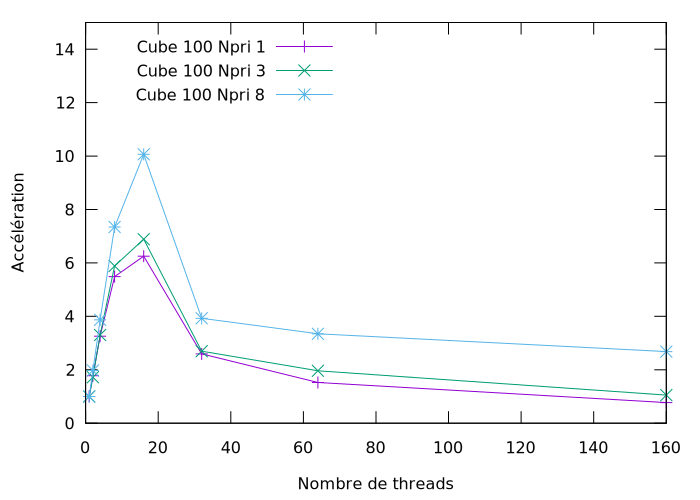
\includegraphics[width=0.48\textwidth]{res_facto_ft_manu}
        }
        \subfigure[Interleave.]{
          \label{fig:res_facto_inter_manu}
          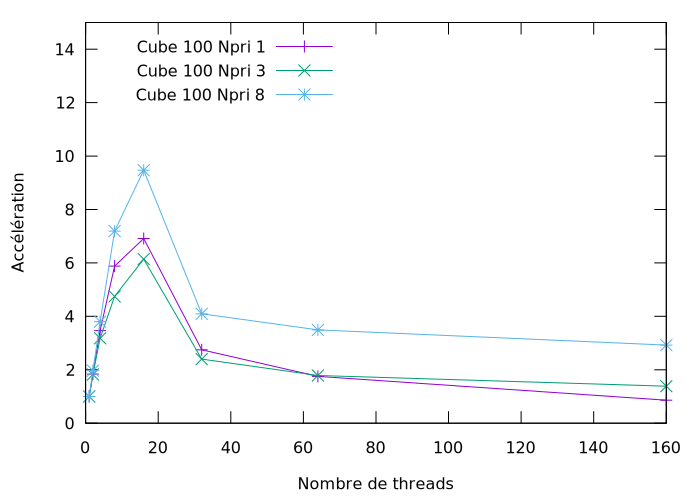
\includegraphics[width=0.48\textwidth]{res_facto_inter_manu}
        }
        \subfigure[NATaS.]{
          \label{fig:res_facto_nas_manu}
          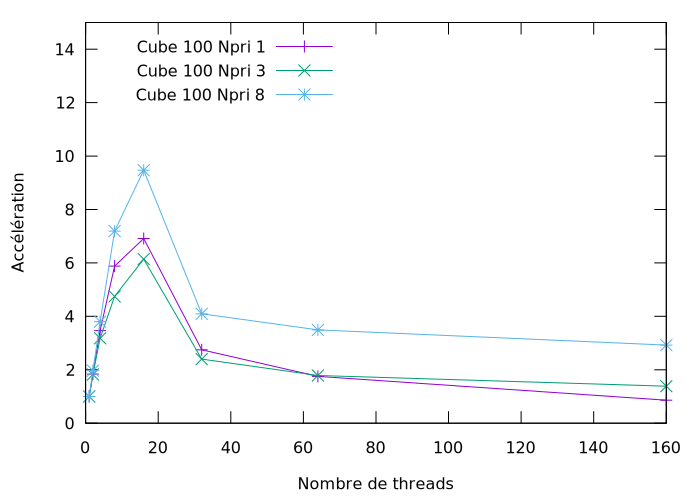
\includegraphics[width=0.48\textwidth]{res_facto_nas_manu}
        }
        \subfigure[MPI.]{
          \label{fig:res_facto_mpi_manu}
          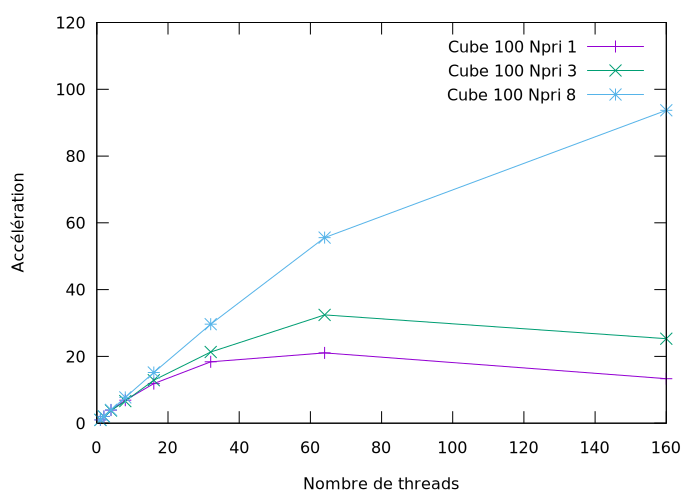
\includegraphics[width=0.48\textwidth]{res_facto_mpi_manu}
        }
    \end{center}
    \caption{Performances de la factorisation ILU(0) sur Manumanu.}
\end{figure}

%%%%%%%%%%%%%%%%
% TRSV
%%%%%%%%%%%%%%%%

%   (-_-)   %
\begin{figure}[p]
     \begin{center}
        \subfigure[First touch.]{
          \label{fig:res_trsv_ft_rostand}
          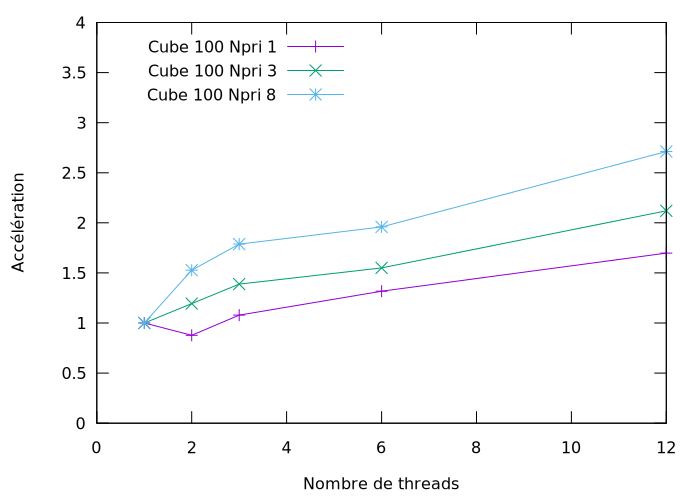
\includegraphics[width=0.48\textwidth]{res_trsv_ft}
        }
        \subfigure[Interleave.]{
          \label{fig:res_trsv_inter_rostand}
          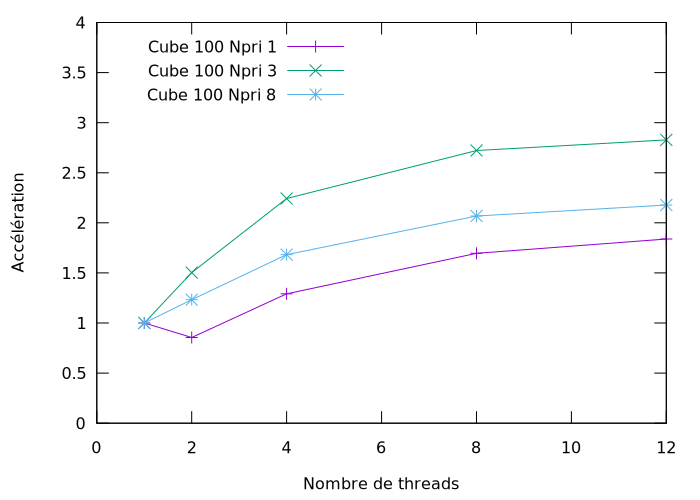
\includegraphics[width=0.48\textwidth]{res_trsv_interleave}
        }
        \subfigure[NATaS.]{
          \label{fig:res_trsv_nas_rostand}
          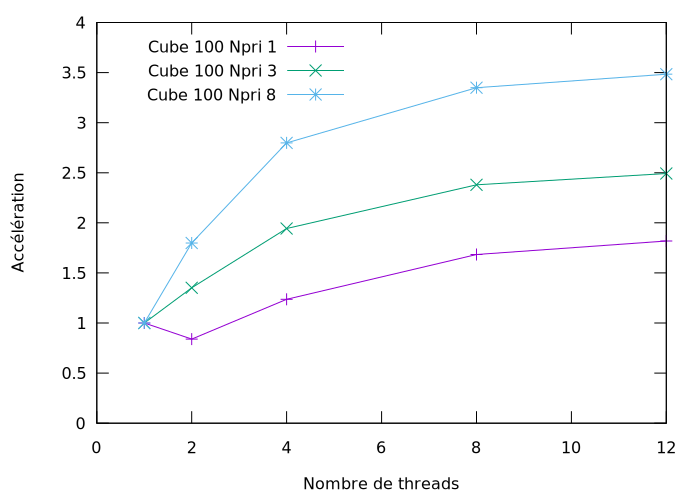
\includegraphics[width=0.48\textwidth]{res_trsv_nas}
        }
        \subfigure[MPI.]{
          \label{fig:res_trsv_mpi_rostand}
          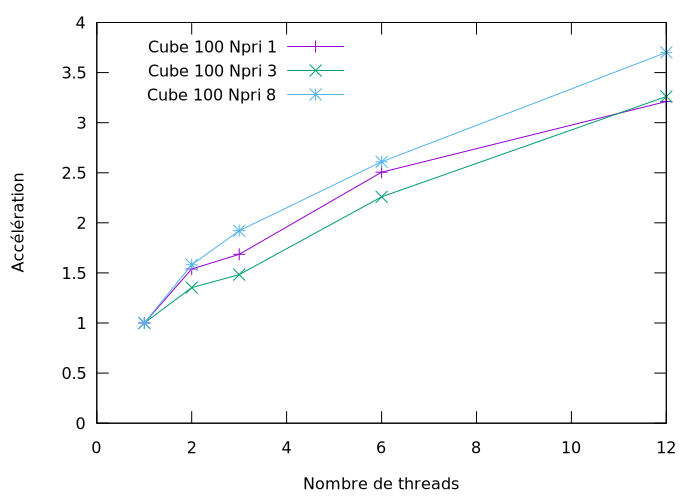
\includegraphics[width=0.48\textwidth]{res_trsv_mpi_numa}
        }
    \end{center}
    \caption{Performances de la résolution triangulaire sur Rostand.}
\end{figure}

%   (-_-)   %
\begin{figure}[p]
     \begin{center}
        \subfigure[First touch.]{
          \label{fig:res_trsv_ft_manu}
          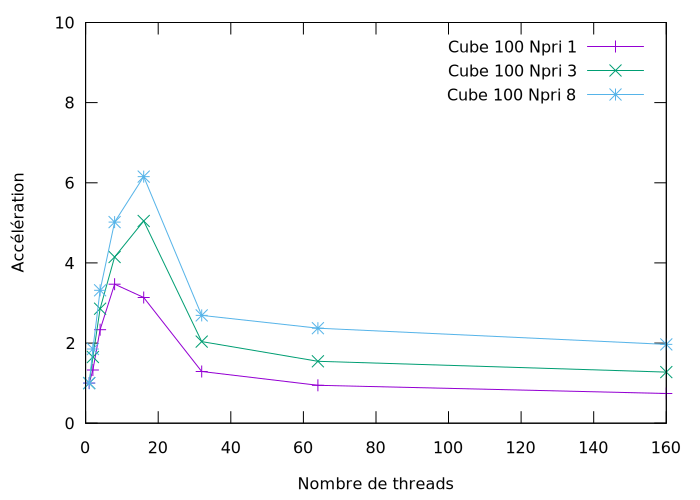
\includegraphics[width=0.48\textwidth]{res_trsv_ft_manu}
        }
        \subfigure[Interleave.]{
          \label{fig:res_trsv_inter_manu}
          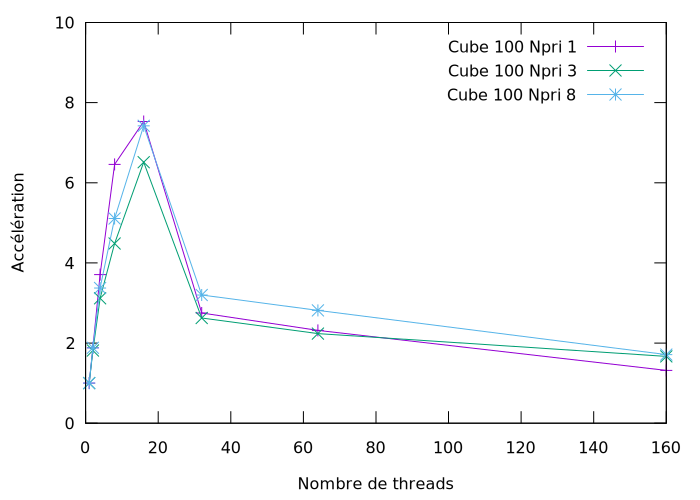
\includegraphics[width=0.48\textwidth]{res_trsv_inter_manu}
        }
        \subfigure[NATaS.]{
          \label{fig:res_trsv_nas_manu}
          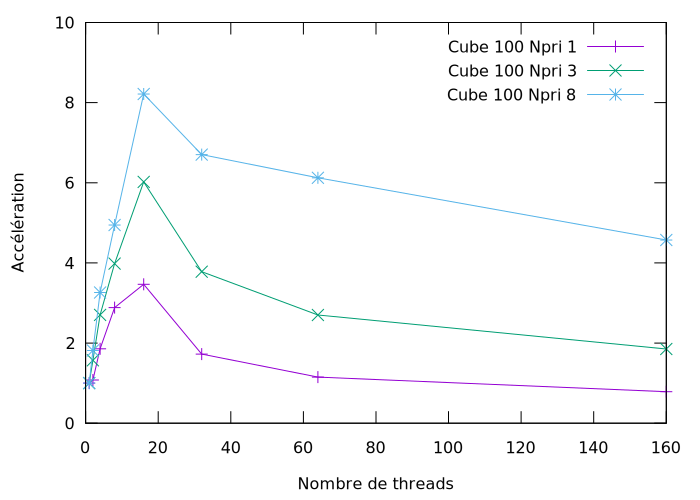
\includegraphics[width=0.48\textwidth]{res_trsv_nas_manu}
        }
        \subfigure[MPI.]{
          \label{fig:res_trsv_mpi_manu}
          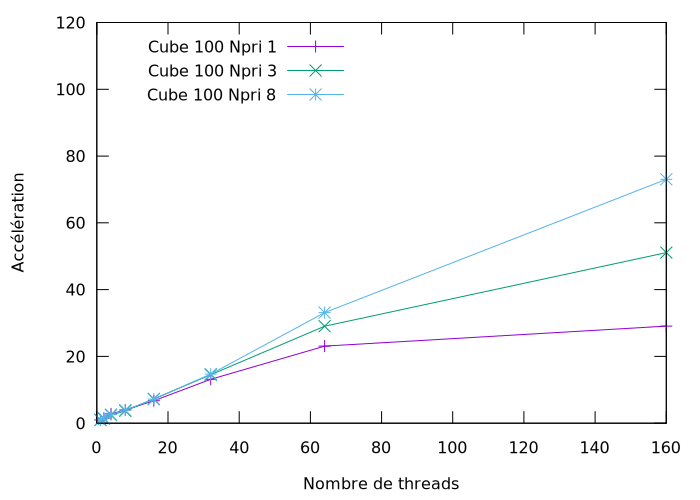
\includegraphics[width=0.48\textwidth]{res_trsv_mpi_manu}
        }
    \end{center}
    \caption{Performances de la résolution triangulaire sur Manumanu.}
\end{figure}

%-------------------------------
\subsubsection{\'Equilibrage automatique NUMA}
L'équilibrage automatique des pages mémoires ne donne pas de bonnes performances sur la factorisation (Fig.~\ref{fig:res_facto_frep}).
%
Cette méthode d'allocation est la moins efficace de toutes.
%
Avec un nombre suffisant d'itérations, l'allocation interleave donne les mêmes performances que l'allocation first touch.
%
L'utilisation de NATaS reste la solution qui donne les meilleures performances.

%   (-_-)   %
\begin{figure}
  \centering
  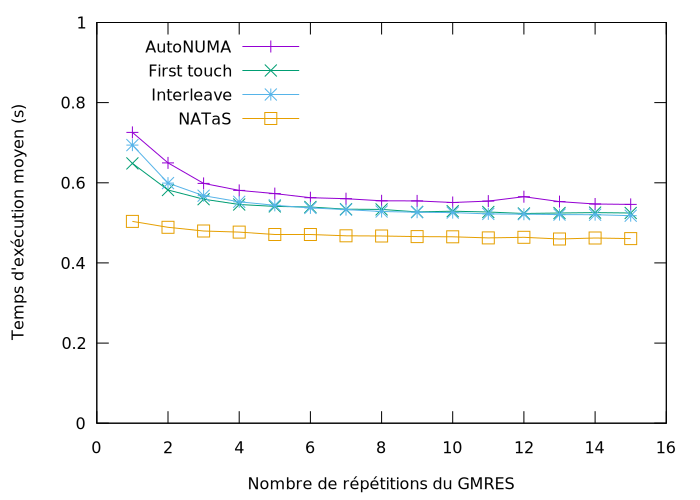
\includegraphics[width=0.7\textwidth]{res_facto_frep}
  \caption{Temps moyen d'une factorisation sur Linux 3.18 en mémoire partagée avec 12 coeurs. Nous utilisons une matrice représentant un cube 100 avec 8 variables primaires.}
  \label{fig:res_facto_frep}
\end{figure}
Par contre, la résolution triangulaire se comporte comme le SpMV (Fig.~\ref{fig:res_trsv_frep}).
%
La politique d'allocation autoNUMA offre des performances intermédiaires aux politiques d'allocations first touch et interleave.
%
Encore une fois, l'utilisation de NATaS est la plus efficace.

%   (-_-)   %
\begin{figure}
  \centering
  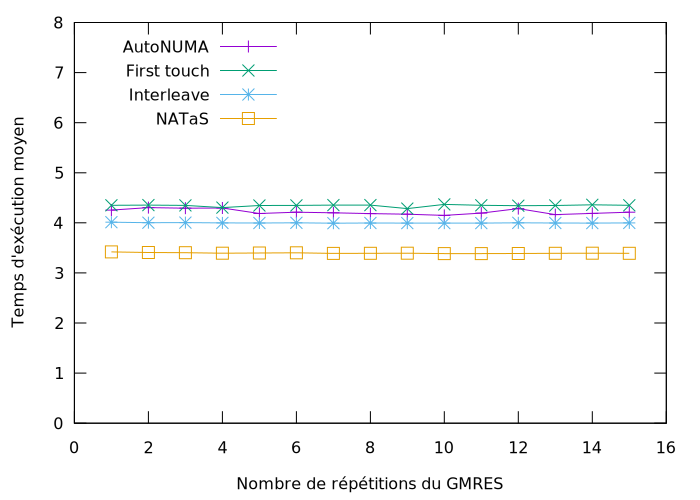
\includegraphics[width=0.7\textwidth]{res_trsv_frep}
  \caption{Temps moyen d'une résolution triangulaire sur Linux 3.18 en mémoire partagée avec 12 coeurs. Nous utilisons une matrice représentant un cube 100 avec 8 variables primaires.}
  \label{fig:res_trsv_frep}
\end{figure}

% -------------------------------
